\documentclass{article}
\usepackage{graphicx}
\usepackage{hyperref}
\usepackage{caption}
\usepackage{subcaption}
\usepackage{mathtools}
\usepackage[dutch]{babel}

\begin{document}

\begin{center}
	\huge{Wiskunde in Kunst}\\
	\LARGE{Opdracht }8 \\
	
	\vspace{2cm}
	
	\Large{De Fibonacci reeks}\\
	
	\vfill
	
	\begin{figure}[Hh]
		\centering
		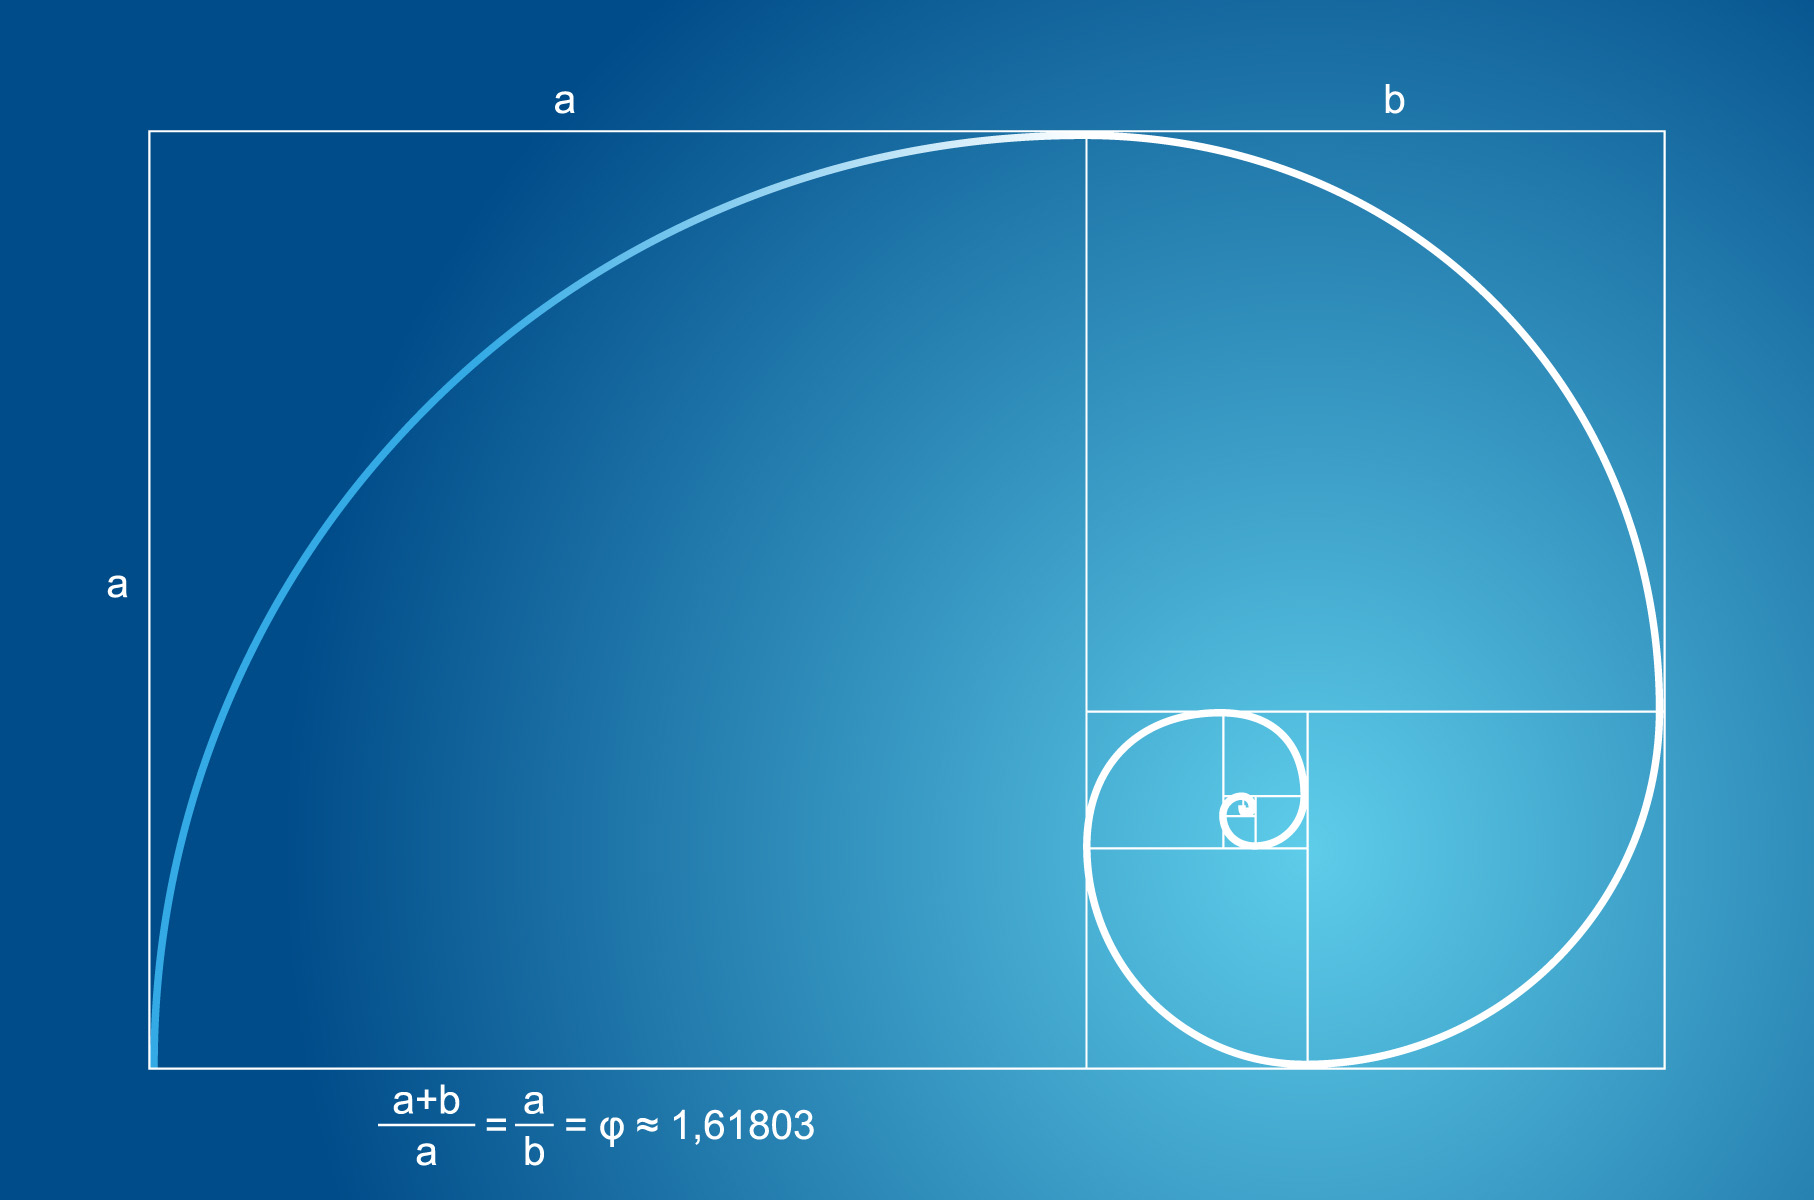
\includegraphics[width=\textwidth]{golden-ratio.jpg}
	\end{figure}
	
	\vfill
	\Large{Marcelo Dias Avelino} \hfill \large{0840416}
\end{center}

\pagebreak

\section{De wiskundige}

De Fibonnaci reeks is een reeks van getallen die genoemd zijn naar de italianse wiskundige Leonardo Pisano Bigollo. Fibonnaci was geboren op 1170, zon van een rijke handelaar genaamd Guglielmo Bonacci. Zijn vader was een simpele dwaas en was bijgenaamd Bonaccio, wat `dwaas' betekende in de idioom destijds. Hieruit is ook de naam Fibonacci onstaan, wat `zoon van een dwaas' betekent. Zijn vader was consul voor Pisa en eigenaar van een handelspost in B\'eja\"ia, een havenstad oost van Algiers, de hoofdstad van Algerije. Als kleine jonge reisde Fibonnaci heel vaak met zijn vader naar Algerije om hem te helpen en tijdens zijn verblijf daar heeft hij de Hindu-Arabische getallen stelsel geleerd. Hij erkende dat deze getallen stelsel veel effienc\"ienter was om mee te rekenen dat de romeinse stelsel dat destijds nog gebruikt werd overal in Europa en besloot om door het hele Mediterranse wereld te reizen om onder de arabische wiskundige meesters te leren.

 In 1202, toen Fibonnaci 32 was, heeft hij alles wat hij heeft geleerd opgeschreven in een boek genaamd \textit{Liber Abaci} (Boek van Berekeningen). Hierdoor was de Hindu-Arabische getallen stelsel bekend geworden in Europa en uiteindelijk compleet overgenomen. Dit boek bepleitte het gebruik van de cijfers 0 t/m 9 en het gebruik van de positiestelsel. 

De positiestelsel is de systeem dat cijfers hun waarde toekent gebaseerd op hun positie binnen een getal. Dit door elke cijfer te vermenigvuldigen met het aantal symbolen gebruikt in het getallenstelsel, in dit geval 10 symbolen (0 - 9), tot de macht te verheffen van de positie van het getal (beginnend op 0), en alle waardes uiteindelijk bij elkaar op te tellen. Bijv. bij het getal \textit{153}, de positie van het getal 3 bepaalt dat zijn waarde \(3 \times 10^0 = 3\) is, het getal 5 wordt \(5 \times 10^1 = 50\) en het getal 1 wordt \(1 \times 10^2 = 100\). Alles bij elkaar opgeteld komt weer op het getal \(3 + 50 + 100 = 153\) uit.

\begin{figure}[Hh]
	\centering
	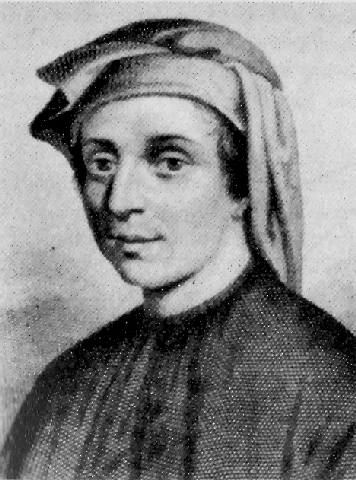
\includegraphics[width=0.3\textwidth]{Fibonacci.jpg}
	\caption{Portret van Fibonnaci door onbekende auteur.}
\end{figure}

% die als volgt eruit ziet: 

% \textit{1, 1, 2, 3, 5, 8, 13, 21, 34, 55, 89, 144, ...} .

% Deze reeks volgt de volgende formule:

% \(k_{n+1} = n^2 + k_n^2 - k_{n-1}\)

\pagebreak

\begin{thebibliography}{9}

\bibitem{}
	\url{http://en.wikipedia.org/wiki/Circle_Limit_III}
	
\end{thebibliography}

\end{document}
